 \section{System sygnałów i slotów}
        Wprowadzenie tego rodzaju funkcjonalności rozegrało niebagatelne znaczenie w popularności frameworka QT. W przygotowanej na potrzeby opisywanego projektu aplikacji, system sygnałów i slotów pełni kluczową rolę w jej funkcjonowaniu. Na listingu \ref{code:app_qt_connections} został umieszczony fragment programu odpowiadającego za przypisanie sygnałów produkowanych przez liczne elementy interfejsu użytkownika do specjalnie przygotowanych na tę potrzeby funkcji. Nie trudno sobie wyobrazić jak wiele pracy jest w stanie oszczędzić proste łączenie sygnałów ze slotami w porównaniu ze żmudną implementacją karkołomnych rozwiązań na własną rękę. Pozwala to także na omijanie sytuacji, w której nie jeden programista sięgnąłby po rozwiązanie jakim jest wielowątkowość. Sposób działania tego rozwiązania przedstawiony jest na rysunku \ref{fig:s&s}.
        
       \begin{figure}[ht]
          \centering
          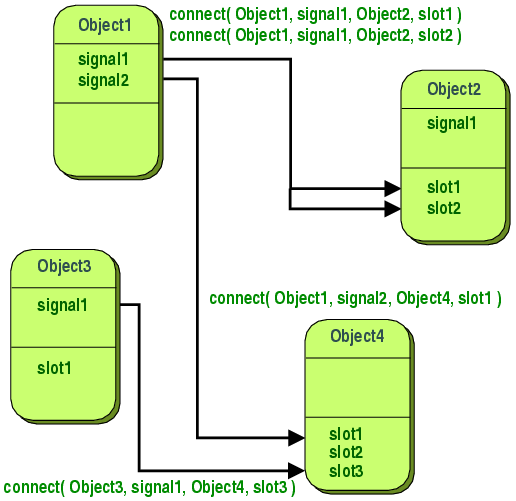
\includegraphics[width=0.6\textwidth]{img/abstract-connections.png}
          \caption{System sygnałów i slotów \cite{qt_s&s_fig}}
          \label{fig:s&s}
        \end{figure}     
        
        \begin{kod}
          \inputminted[firstline=18, lastline=39]{cpp}{app/listings/mainwindow.cpp}
          \caption{Użycie systemu sygnałów i slotów}
          \label{code:app_qt_connections}
        \end{kod}
        
